%! suppress = MissingImport
\section{Introduction}
In fact, there is no uniform definition of modern programming language.
Different researchers define it through different aspects, such as finding
the connection between software engineering and modern programming language,
or elaborate around "abstraction".
The above statements are correct within their own scope, and the scope of
application is expanded again.
Through studying a variety of definition intersections, more universal modern
programming language definition is obtained.
An obvious fact is that with the continuous deepening of programming language practice,
the definition of modern programming language is constantly changing,
because programming language is the theory of close combination of
practice and theory.
Although its definitions are constantly changing,
some core contents are always unchanged.
Here are several characteristics of modern programming languages.


1. The essence is greater than the form. It should provide descriptive grammatical structures instead of telling the machine what the machine should do. It is essentially an abstraction to the function of the machine.

2. Semantic consistency. For similar grammar structures, similar grammatical characteristics should be available.

3. Grammar self -lifting. For non -core grammar characteristics, on the basis of following semantic consistency, it should be composed of the core grammar characteristics.

4. Multi -paradigm. Provide a variety of programming paradigms without forcing users to use specific programming paradigms.

5. Check it during compilation. For potential errors, it should be prevented during the compilation period, rather than reporting at runtime.


The programming language has a considerable time limit. For different programming languages of different eras, although they are in line with the characteristics of the above -mentioned modern programming language, one of them is still more "outdated" compared to the other. This is because the above principles are conflict in time dimension. In fact, the essence is greater than the form of programming language abstraction that meets the grammatical characteristics of specific application scenarios, and the needs of the application scenario will gradually change over time, because the application scenarios will be upgraded by technical iteration. At this time, if you want to add new grammar characteristics to the original programming language, it is easy to destroy the principles of grammar self -lifting and semantic consistency. Therefore, a better solution at this time is to design a new programming language, and consider meeting new needs from the language design.

However, there are some factors that hinder the progress of the elimination of programming language. The programming language takes a long time from the prototype to the large -scale application. During this time, the programming language will gradually improve your programming language ecosystem. The programming language ecology is like a dense network. Once the programming language starts to apply large -scale application, it is almost impossible to completely eliminate the programming language. For developing computer application systems, the most ideal state is that the new programming language can be compatible with the old programming language, so that the new programming language can inherit the ecology of the old programming language. A typical example is C and C ++. However, due to the existence of some possibilities, many times the new programming language cannot be compatible with the old programming language. At this time, the compatibility of the programming language ecosystem can be achieved through the virtual machine, but it is limited to the new programming language and the old programming language. A typical example of the same virtual machine is Java and Kotlin. In addition, there is a more universal method that the new programming language realizes the data interface of the old programming language. Most of the language and the interaction of C/C ++ are completed, but there will be greater functional restrictions. Finally, it is a method that does not depend on the specific implementation of programming languages. By introducing a third -party protocol to achieve low -coupled compatibility, a typical example is the RPC framework of each language. Each programming language is compatible with some past programming languages, which is also inevitable.

\begin{figure}[htbp]
    \centerline{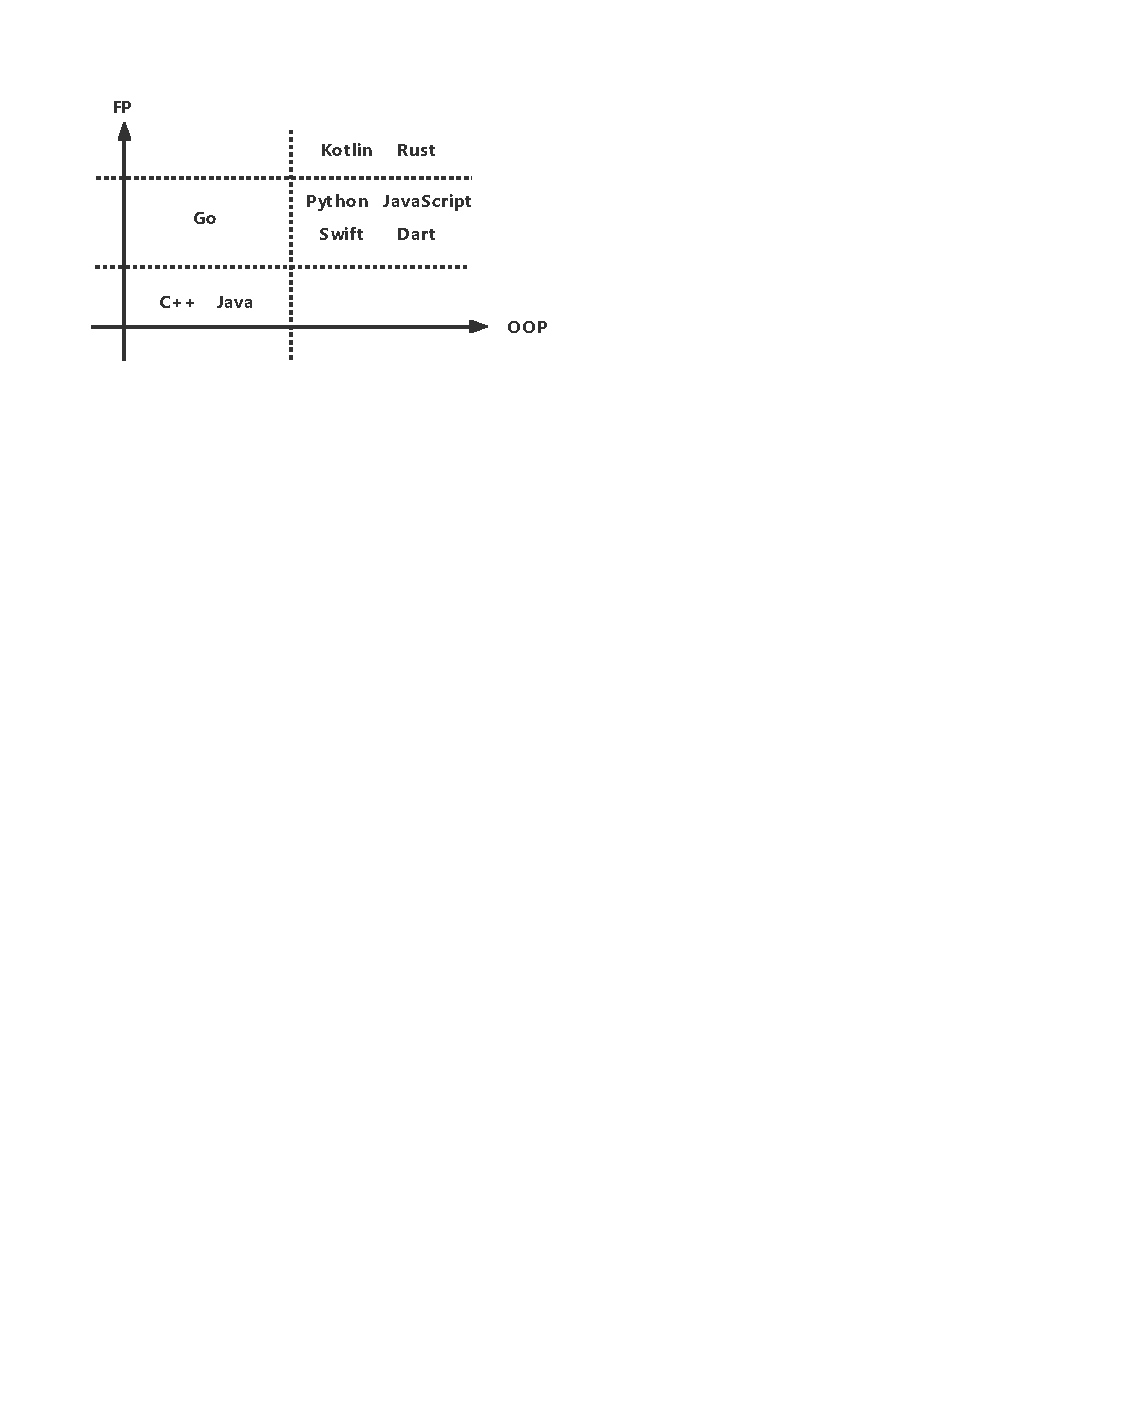
\includegraphics[scale=0.8]{figures/paradigm}}
    \caption{demo}
    \label{fig:sample_figure}
\end{figure}

\begin{table}[htbp]
    \caption{demo}
    \label{tab:demo}
    \begin{center}
        \begin{tabular}{lrrrr}
            \toprule
            lang      & n    & size(B) & cpu(s) & mem(KB) \\
            \midrule
            cpp-clang & 4000 & 822     & 0.880  & 1552    \\
            cpp-gcc   & 4000 & 822     & 0.881  & 1192    \\
            dart-aot  & 4000 & 454     & 10.276 & 17380   \\
            dart-jit  & 4000 & 454     & 10.096 & 148084  \\
            go        & 4000 & 823     & 1.260  & 2420    \\
            java      & 4000 & 665     & 1.827  & 34352   \\
            js-node   & 4000 & 373     & 8.763  & 42540   \\
            python3   & 4000 & 688     & 46.273 & 12172   \\
            rust      & 4000 & 868     & 0.757  & 4388    \\
            swift     & 4000 & 394     & 1.661  & 6240    \\
            \bottomrule
        \end{tabular}
    \end{center}
\end{table}

\begin{table*}[htbp]
    \caption{demo}
    \label{tab:demo1}
    \begin{center}
        \begin{tabular}{ccccccc}
            \toprule
            Language & Encapsulation & Inheritance & Composition & Delegation &
            Polymorphism & Everything is object \\
            \midrule
            Python     & \Checkmark & \Checkmark & \Checkmark & \Checkmark & \Checkmark & \Checkmark \\
            Java       & \Checkmark & \Checkmark & \Checkmark & ×          & \Checkmark & ×          \\
            C++        & \Checkmark & \Checkmark & \Checkmark & ×          & \Checkmark & ×          \\
            JavaScript & \Checkmark & \Checkmark & \Checkmark & ×          & \Checkmark & \Checkmark \\
            Go         & \Checkmark & ×          & \Checkmark & \Checkmark & \Checkmark & ×          \\
            Swift      & \Checkmark & \Checkmark & \Checkmark & ×          & \Checkmark & \Checkmark \\
            Dart       & \Checkmark & \Checkmark & \Checkmark & ×          & \Checkmark & \Checkmark \\
            Rust       & \Checkmark & ×          & \Checkmark & \Checkmark & \Checkmark & \Checkmark \\
            Kotlin     & \Checkmark & \Checkmark & \Checkmark & \Checkmark & \Checkmark & \Checkmark \\
            \bottomrule
        \end{tabular}
    \end{center}
\end{table*}


